\documentclass[a4paper,twoside,12pt]{report}   	% use "amsart" instead of "article" for AMSLaTeX format
\usepackage{geometry}                		% See geometry.pdf to learn the layout options. There are lots.
\geometry{letterpaper}                   		% ... or a4paper or a5paper or ... 
%\geometry{landscape}                		% Activate for rotated page geometry
%\usepackage[parfill]{parskip}    		% Activate to begin paragraphs with an empty line rather than an indent
\usepackage{graphicx}				% Use pdf, png, jpg, or eps§ with pdflatex; use eps in DVI mode
								% TeX will automatically convert eps --> pdf in pdflatex		
\usepackage{amssymb}



% customize
\usepackage[utf8]{inputenc}
\usepackage[T1]{fontenc}
\usepackage{lmodern}
\usepackage[Glenn]{fncychap}
\usepackage{fancyvrb,xcolor}
\usepackage{moreverb}
\usepackage{amsmath}
\usepackage{amssymb}
\usepackage{mathrsfs}
\usepackage[french]{babel}
\usepackage{graphicx, float}
\usepackage{multirow}
\usepackage{enumitem, pifont}
\usepackage{multicol}
\usepackage{algorithm,algorithmic}
\usepackage{pdfpages}
\usepackage{eqparbox,array}
\usepackage{longtable}
%\usepackage[acronym]{glossaries}
\usepackage[toc]{glossaries}

\newcommand{\fonction}[5]
{
  \begin{array}{lrcl}
    #1:&#2& \rightarrow& #3 \\
    & #4&\mapsto&#5
  \end{array}
}
\newtheorem{theo}{\textbf{Theorem}}[section]
\newtheorem{prop}{\textbf{Property}}[section]
\newenvironment{proof}[1][Proof:]
{\begin{trivlist} \item[\hskip \labelsep  {\bfseries #1}]}
{\end{trivlist}}
\newenvironment{proofInd}[1][Proof indications:]
{\begin{trivlist} \item[\hskip \labelsep  {\bfseries #1}]}
{\end{trivlist}}
\renewcommand\algorithmiccomment[1]{%
  \hfill  \eqparbox{COMMENT}{\scriptsize \textit{#1}}%
}
\newcommand\LONGCOMMENT[1]{%
  \hfill\#\ \begin{minipage}[t]{\eqboxwidth{COMMENT}}#1\strut\end{minipage}%
}
% end customize

\usepackage{url}
\usepackage{titling}

% glossaires and acronyms
\makeglossaries
\newacronym{fpm}{FPM}{Frequent Pattern Mining}
\newglossaryentry{formula}
{
    name=formula,
    description={A mathematical expression}
}


%opening
\title{ FREQUENT PATTERN (FP) GROWTH ALGORITHM}
\author{BINELI OLA Mathilda Maguy 17T2215,\\ DJIEMBOU TIENTCHEU Victor Nico 17T2051,\\KENFACK TEMGOUA Vanessa 17J2871\\Coordonateur (Université de Yaoundé I): Dr TSOPZE NORBERT\\ \ \ \ \ }


%\date{}							% Activate to display a given date or no date

\linespread{1.3}

\begin{document}
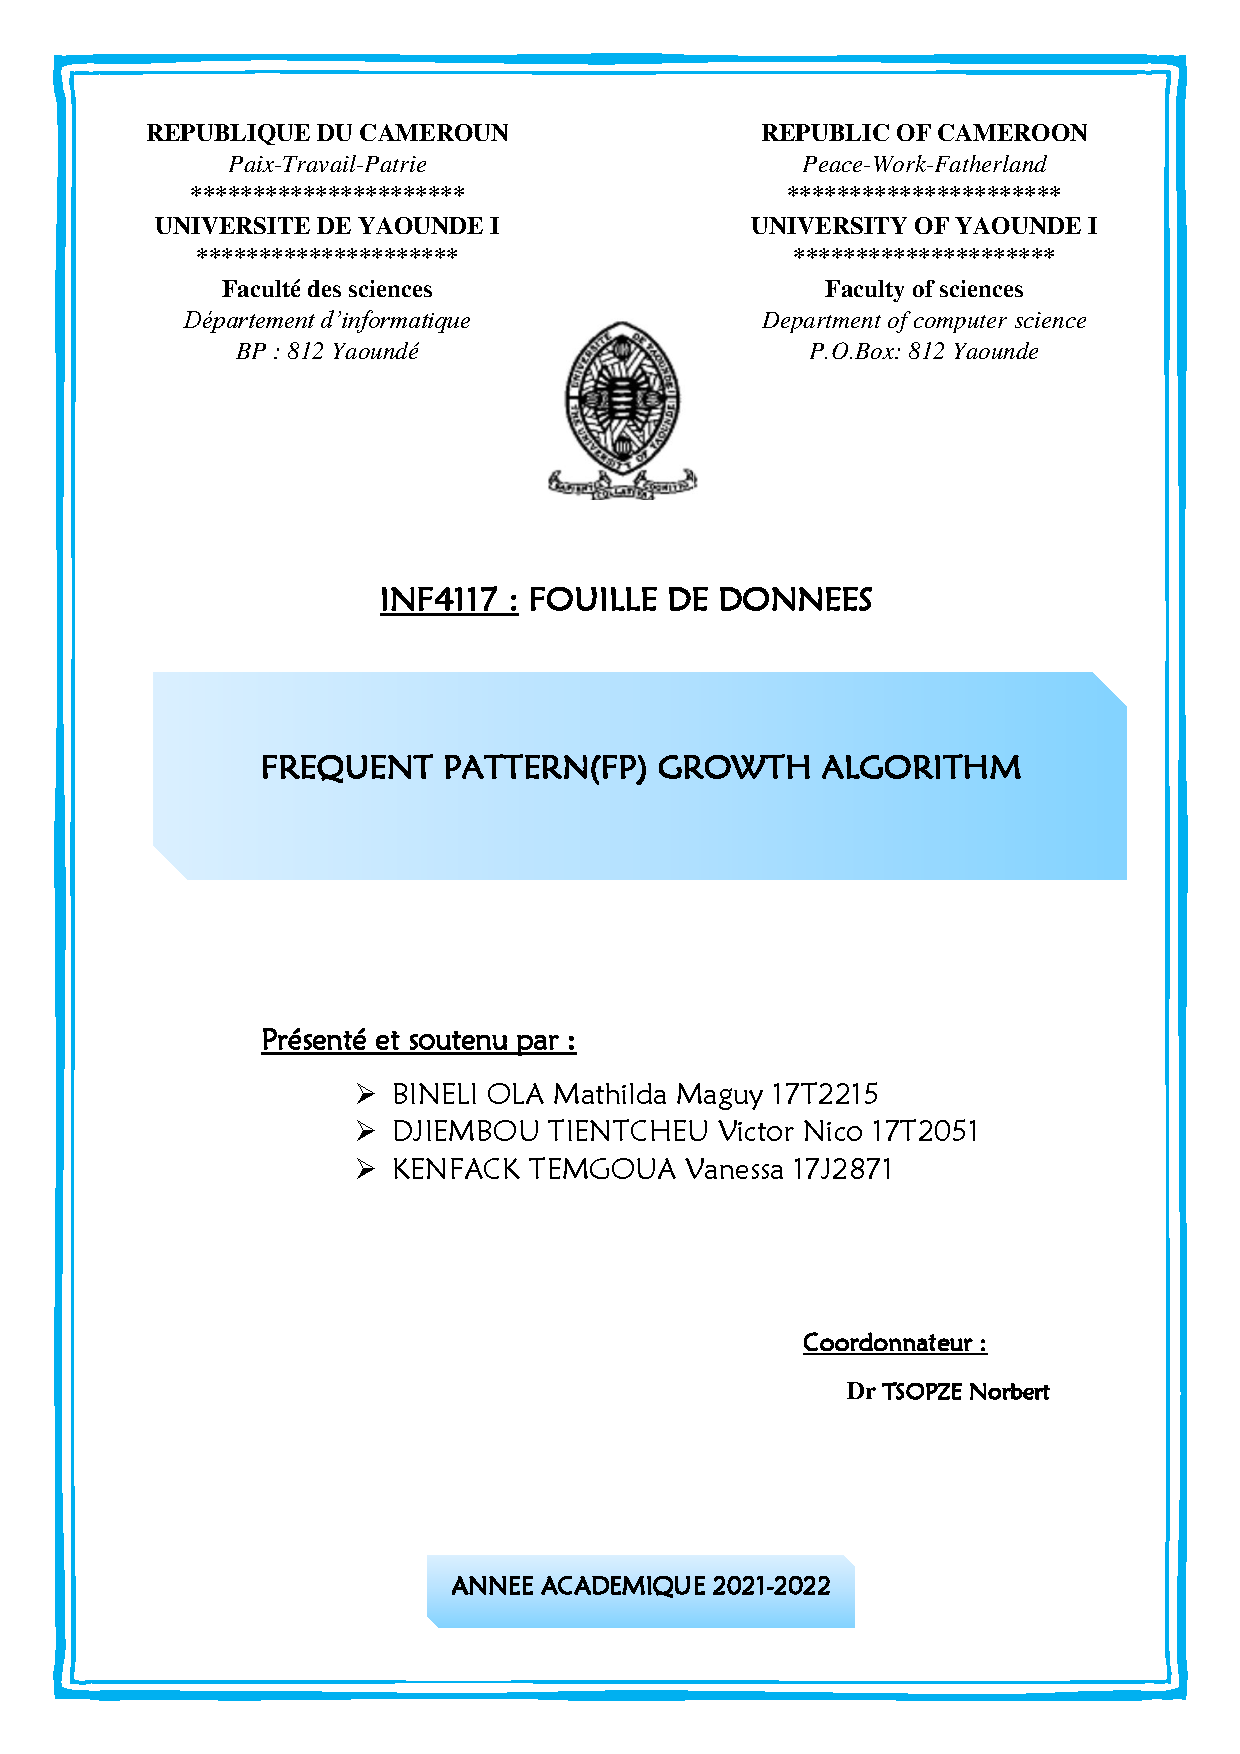
\includepdf[pages={1}]{couverture4117.pdf}
\maketitle


\newpage

\pagenumbering{roman}
\tableofcontents
\listoftables
\listoffigures  % table des figures

\newpage
\pagenumbering{arabic}

% first chapter

\chapter{Introduction}
\label{chapitre introductif}

\section{Introduction}
\par L'extraction de connaissance dans les bases de données, également appelé \textbf{data mining}, désigne le processus permettant d'extraire des informations et des connaissances utiles qui sont enfouies dans les bases de données, les entrepôts de données (data warehouse) ou autres sources de données.
\par Depuis sa création, le Data Analytique joue un rôle important dans le processus de prise de décision, du coup plusieurs algorithmes \acrfull{fpm} ont été développés pour améliorer les performances d'extraction.
\par Durant ce chapitre, nous nous intéresserons à l'algorithme de croissance de motifs fréquents dans l'extraction de connaissances.
\par Le but de cette étude est de présenter tout d'abord ce que s'est que \textbf{l'Algorithme de croissance de Motifs fréquents} (\textit{FP Growth Algorithm}, en anglais), quels sont les atouts? et quels sont ses limites?
\Glspl{formula}
\section{Définitions}
\textbf{Items:}\\ Est tout objet, article, attribut, littéral appartenant à un ensemble fini d'éléments distincts $I = \{x_1, x_2, x_3, \dots, x_n\}$. En outre, il s'agit d'un ensemble d'attribut de la base de données transactionnelle.
\par \textbf{Itemset:}\\ C'est un ensemble de \textbf{N} items.
\par \textbf{Itemset Frequent:}\\ On dit qu'un itemset est fréquent si et seulement si son support est supérieur à un support minimum définit par l'utilisateur.
\par \textbf{support minimal:}\\ Noté \textbf{Minsup} est le nombre minimum d'occurence d'un itemset pour être considéré comme fréquent.
\par \textbf{Transaction:}\\ Soit $I = \{i_1, i_2, \dots, i_m\}$ un ensemble d’items, D une BD de transactions o\`u chaque transaction T est un sous ensemble de I.
\par \textbf{Base de données transactionnelle:}\\ 
\par \textbf{règle:}\\ Une r\`egle d’association est une implication de la forme $A \Longrightarrow B$ où  A \sqsubseteq I , B ⇢ I et A \ B = {}
\par \textbf{Confiance:}\\ 
%\section{ok}
%\subsection{}
\clearpage

\printglossary[title=Special Terms, toctitle=List of terms]

\end{document}  